
\section{The Totem Platform: AI and AR in Digital Art}

\begin{figure}[h]
    \centering
    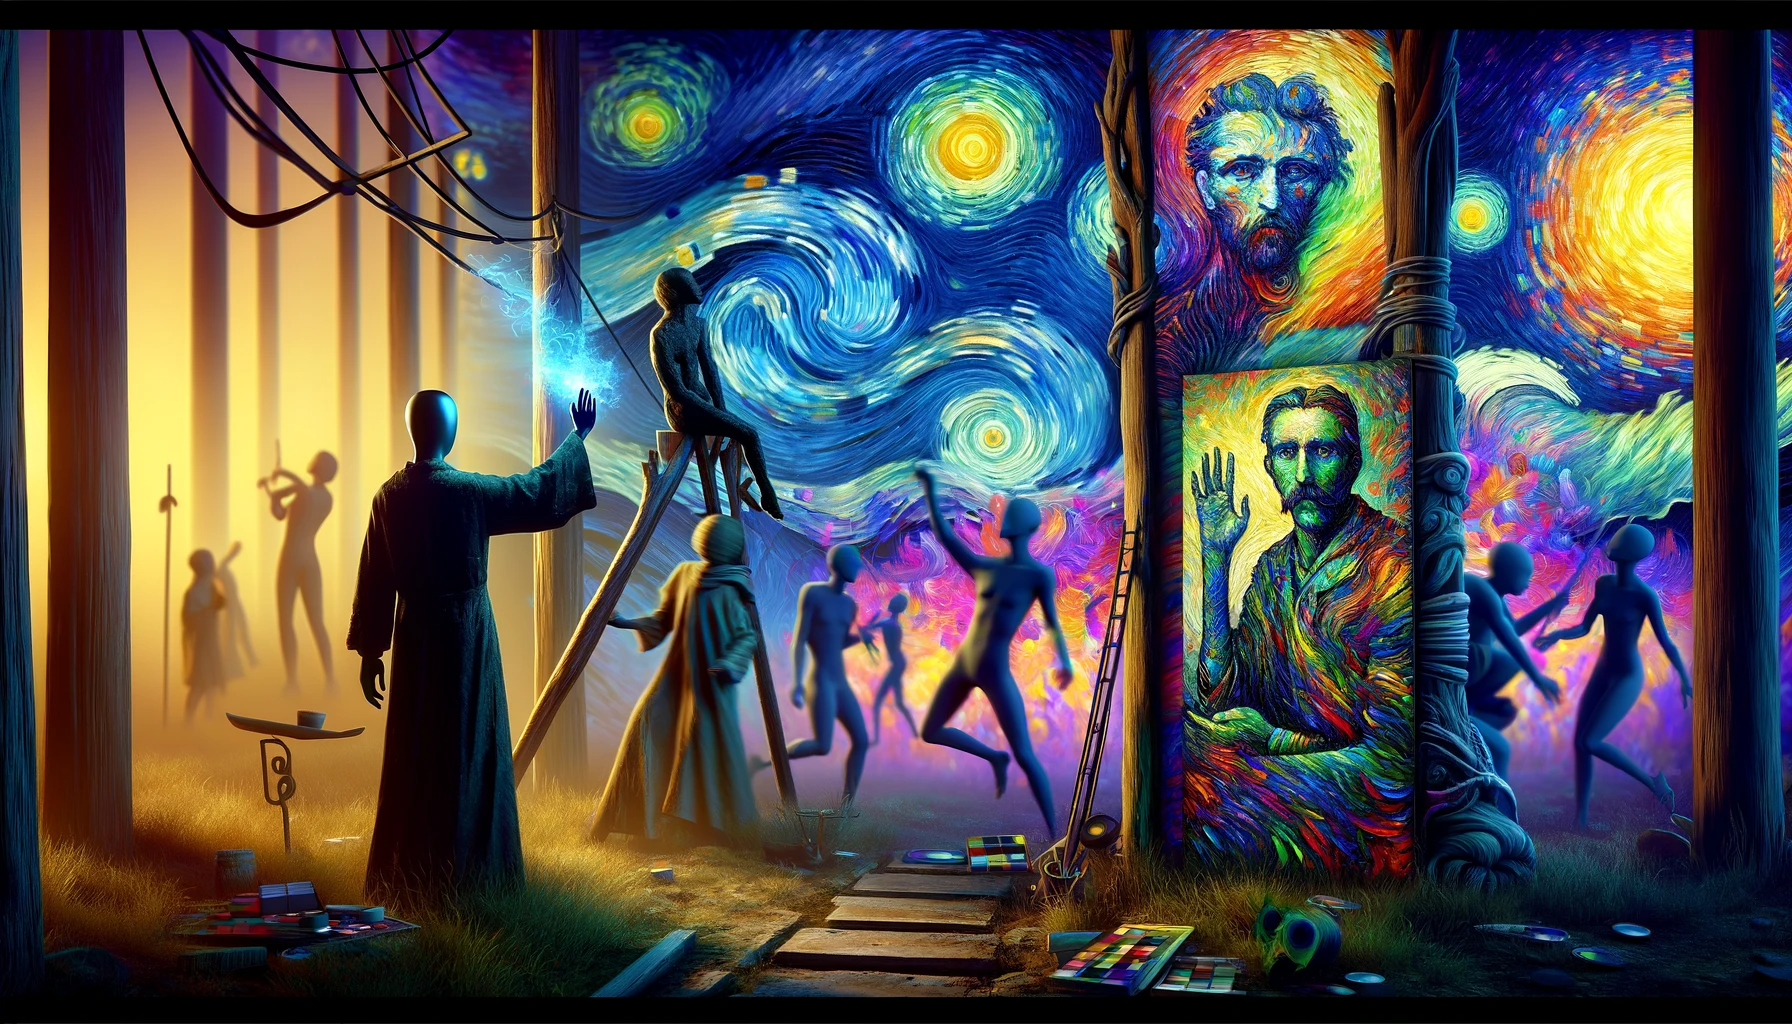
\includegraphics[width=\textwidth]{totemBanner.png}
    \caption{The spirit of the Totem platform.}
    \vspace{0.1cm}
    \label{fig:spiritofTotem}
\end{figure}

The Totem platform stands at the forefront of combining Artificial Intelligence (AI) and Augmented Reality (AR) to offer a unique and innovative way of creating digital art.
This platform integrates two cutting-edge technologies, SDXL Turbo\cite{sauer2023adversarial} and the First Order Motion model\cite{Siarohin_2019_NeurIPS}, to transform basic sketches into interactive AR experiences.
The Backbones of the Totem platform is GOSAI\cite{gosai2022}, an AR framework that propels Augmented Reality applications to new heights.

It starts with a user's simple drawing. Using SDXL Turbo, a powerful diffusion model developed by Stability AI, these drawings are quickly turned into detailed AI-generated images.
This step elevates the initial sketch beyond its original form, providing a new level of artistic detail and creativity. The process doesn't stop there.
The Totem platform then employs the First Order Motion model to bring these images to life.
This model adds realistic movements and expressions to the AI-generated art, creating characters that can move and interact within an AR setting.
This step is crucial in making the art not just more engaging but also more immersive.
The Totem platform is more than just a tool; it's a glimpse into a new way for creators to interact with their art and for audiences to experience stories in a more engaging manner.


\subsection{Exploring AI and Creativity in HCI}

\begin{figure}[h]
    \centering
    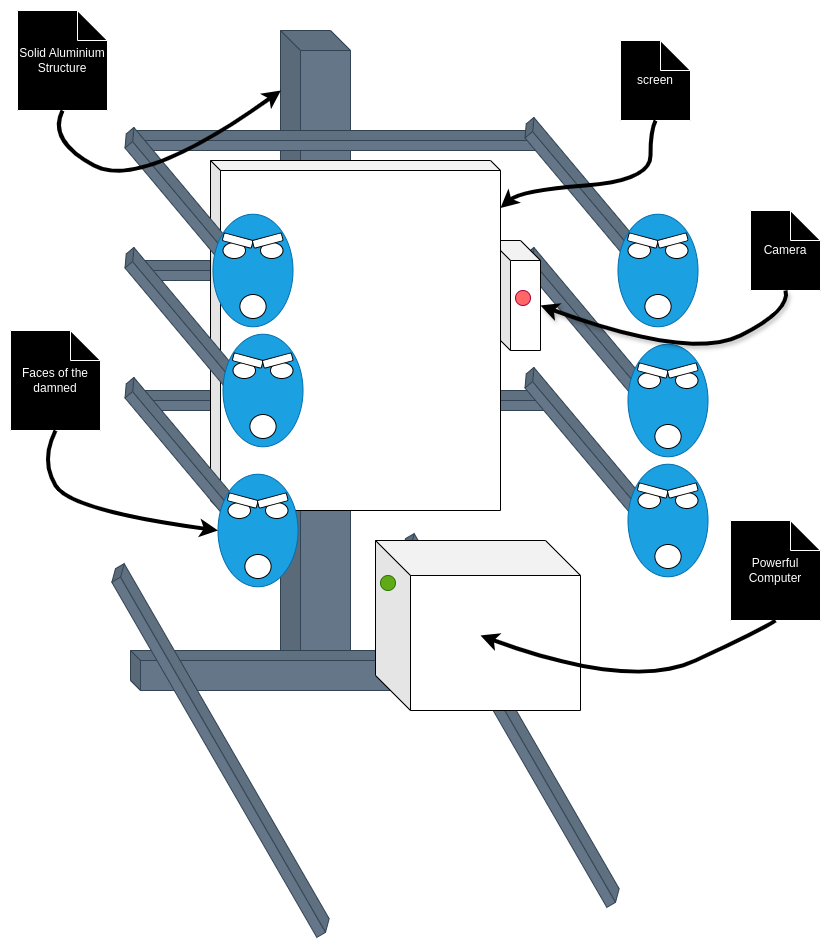
\includegraphics[width=\textwidth/2]{totem.drawio.png}
    \caption{Simplified representation of the Totem platform.}
    \vspace{0.1cm}
    \label{fig:totemImage}
\end{figure}

The \textbf{AI Totem} project is an exploration of how Artificial Intelligence (AI) fits into the creative side of Human-Computer Interaction (HCI).
By combining AI with Augmented Reality (AR), the platform offers a new way to create and experience digital art.
Through advanced AI models such as \textbf{SDXL Turbo} and the \textbf{First Order Motion} deepfake model, the Totem platform turns basic sketches into interactive AR experiences.
Built on the \textbf{GOSAI AR framework}, this system enables artists and developers to explore creative technology in ways that were previously difficult to achieve.

\subsubsection{ Transforming Sketches with AI and AR}

The creative process in the AI Totem platform begins with a simple hand-drawn sketch.
Traditionally, a sketch might be used as a rough guide for more detailed artwork, but here it serves as the starting point for something more complex.
\textbf{SDXL Turbo}, a diffusion model created by Stability AI, processes the sketch and transforms it into a fully detailed AI-generated image.
This model excels at quickly generating high-quality, realistic images from basic inputs, elevating the initial drawing to something far more detailed and visually engaging.

But the platform doesn’t stop at creating static images.
Once the AI-generated image is complete, the \textbf{First Order Motion} model is used to animate it.
This deepfake model brings the image to life by adding movement and expressions.
The result is an animated character that can be placed into an AR environment, interacting with the space and the user. This adds a new layer of immersion, making the art not only visually interesting but also dynamic and interactive.

\subsubsection{ The Role of AR in Enhancing Creative Expression}

Augmented Reality (AR) plays a crucial role in the AI Totem platform, allowing users to engage with their creations in new ways.
AR bridges the gap between the digital and physical worlds, letting users place their AI-generated characters into real-world environments.
Unlike traditional art forms where interaction is limited, AR opens up possibilities for creators to develop work that is interactive and immersive.

One of the challenges in AR is how to balance complexity and usability.
The AI Totem addresses this by integrating AI to handle much of the heavy lifting—interpreting sketches, generating images, and animating them—so that the user can focus on the creative aspects.
AR within the Totem platform doesn't overwhelm users with visual clutter, but instead provides an interface where the interaction is more intuitive, allowing creators to manipulate characters directly with natural gestures or simple controls.

\subsubsection{ AI as a Creative Tool in HCI}

AI in the Totem platform serves as a tool that enhances the creative process.
Traditionally, creating highly detailed artwork or animated characters required significant time and technical expertise.
However, with AI models like SDXL Turbo and First Order Motion, these tasks can be automated or significantly streamlined.
This frees creators to focus on the creative aspects of their work, rather than the technical details of execution.

In the Totem platform, AI functions as a type of \textbf{semantic operator}—interpreting and generating visual elements based on the input it receives.
Just as we discussed in earlier chapters about the role of AI in language processing, the Totem uses AI to understand the intent behind a creator’s sketch and transform it into something more detailed and complex.
This approach simplifies the interaction process, allowing users to achieve complex results with minimal input.

\subsubsection{ Interactive Storytelling and New User Experiences}

The combination of AI and AR in the Totem platform also opens new possibilities for \textbf{interactive storytelling}.
Characters created through this platform are not static—they can be animated, interact with real-world environments, and respond to user actions.
This allows for a more engaging and personalized experience for both creators and audiences.

For example, a creator can design a character that reacts to gestures or interacts with other virtual objects in an AR space.
This makes the storytelling experience dynamic, with the narrative evolving based on user interactions.
The AI Totem is a tool not just for generating art but for creating stories and experiences that feel immersive and responsive.

\subsubsection{ Conclusion}

The \textbf{AI Totem} project highlights how AI and AR can be combined to push the boundaries of creativity in HCI.
By using AI models like SDXL Turbo and First Order Motion, the platform allows users to transform simple sketches into detailed, animated characters that come to life in AR environments.
With the \textbf{GOSAI AR framework} supporting this process, the platform enables creators to explore new ways of expressing ideas, telling stories, and engaging with digital art.
In doing so, AI Totem demonstrates how AI-driven tools can make complex creative tasks more accessible, helping to bridge the gap between technical challenges and artistic expression in the evolving field of HCI.

\subsection{The Implementation of the AI Totem Platform}

The \textbf{AI Totem} platform combines advanced AI models and Augmented Reality (AR) technologies to transform simple sketches into interactive digital art.
The implementation of this platform requires integrating multiple technologies, including the \textbf{GOSAI} framework for AR, \textbf{First Order Motion} for animating characters with deepfake technology, and \textbf{SDXL Turbo} for fast image generation.
This chapter will break down each key component and explain how they come together to power the AI Totem platform.

\subsubsection{ GOSAI: The Backbone of the AR Experience}

At the heart of the AI Totem platform is \textbf{GOSAI}, an open-source framework that simplifies the development of AR applications.
GOSAI enables developers to create AR experiences that seamlessly blend the physical and digital worlds, using an architecture that runs on a variety of devices, from desktops to mobile phones.

GOSAI operates using a \textbf{kernel space and user space architecture}, with drivers in the kernel space handling hardware and computation tasks, and the user space managing the interface and user interactions.
Written in Python and JavaScript, the framework allows developers to integrate AR functionalities such as pose estimation, image recognition, and interaction tracking.
GOSAI is designed to be modular, making it easy to plug in various components, including the AI models used in the Totem platform.

By handling key aspects of AR development, such as camera data processing, pose estimation, and real-time rendering, GOSAI provides a foundation that allows the AI Totem platform to offer interactive and immersive AR experiences.
This framework is responsible for tracking the user's interactions with the generated art, managing the display of the AI-enhanced images, and providing smooth transitions between the physical and digital environments.

\subsubsection{ Deep Fakes: Bringing Art to Life with Motion Models}

The Totem platform integrates \textbf{deepfake technology} to animate the AI-generated images and make them interactive.
While traditional deepfake approaches often use \textbf{Generative Adversarial Networks (GANs)}, such as those in \textbf{DeepFaceLab}, the AI Totem platform employs a different technique—\textbf{motion-based deepfake models} like the \textbf{First Order Motion model}.

The \textbf{First Order Motion model} is ideal for the Totem platform because it requires less computational power than GAN-based deepfakes and can run more efficiently on lightweight devices.
Instead of generating entirely new images, this model deforms existing ones by using keypoints and motion fields. The process begins by identifying sparse trajectories from keypoints, which are then transformed into a dense motion field.
This motion is applied to the original image, animating it in a realistic manner.

\begin{figure}[h]
    \centering
    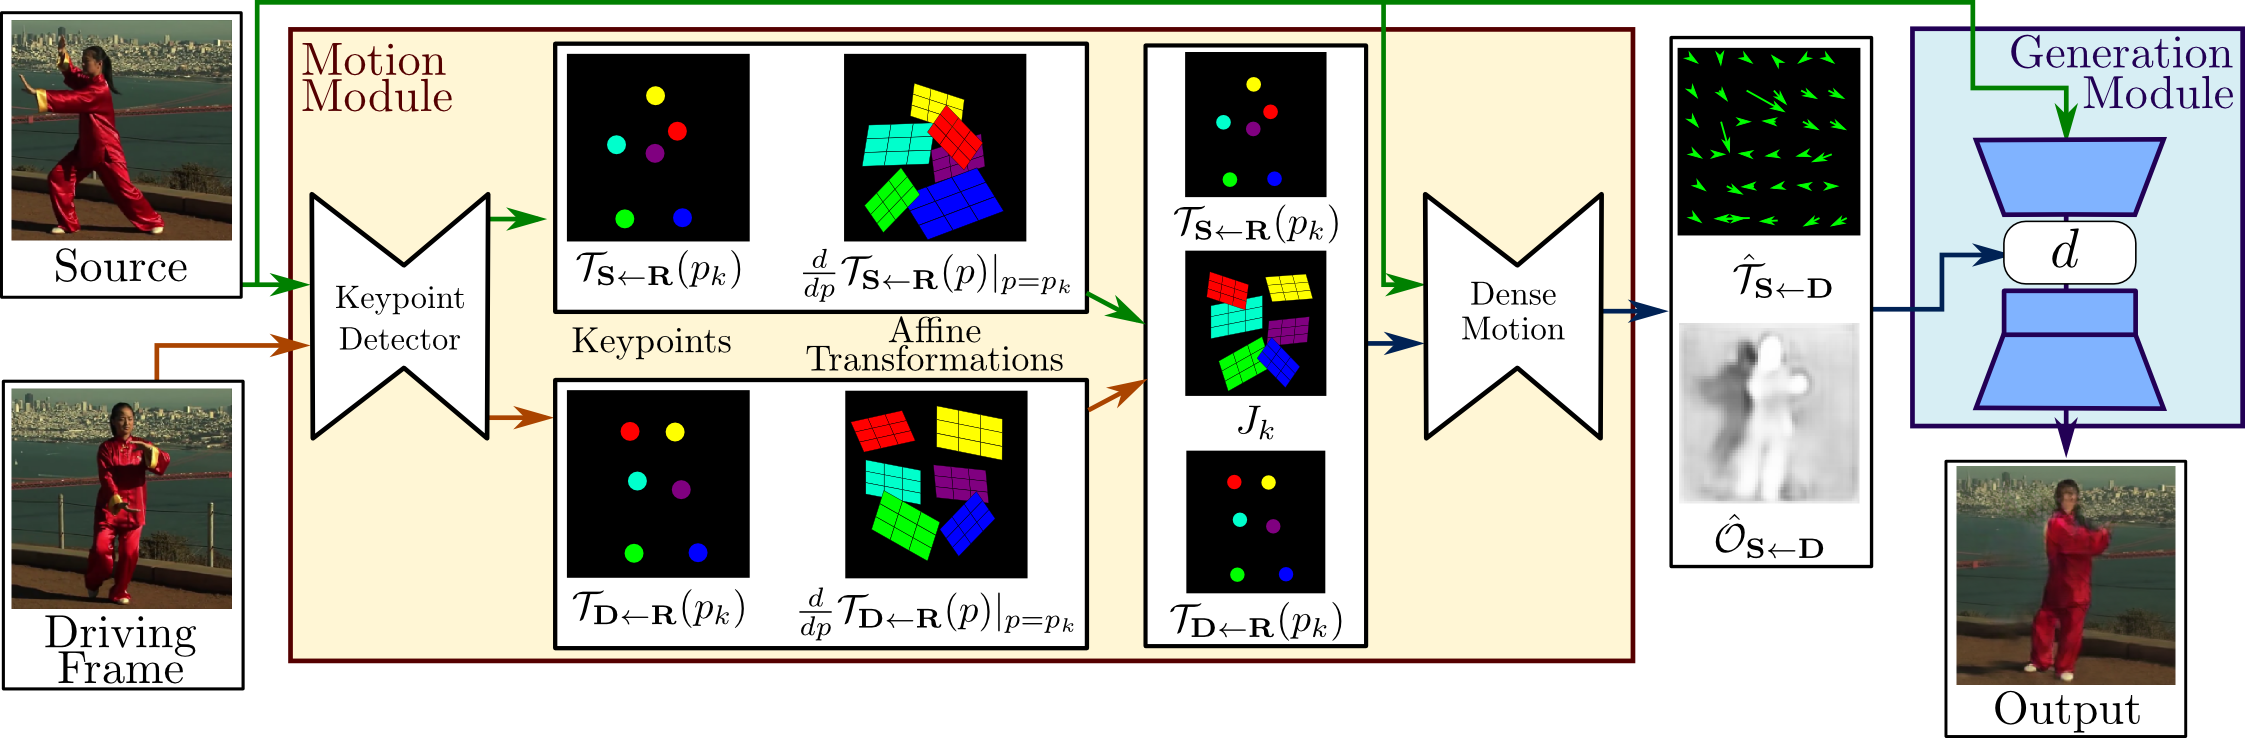
\includegraphics[width=\textwidth]{firstordermotion.png}
    \caption{Architecture of the First Order Motion Model.}
    \vspace{0.1cm}
    \label{fig:firstorderarchitecture}
\end{figure}

This method allows the AI Totem platform to create lifelike animations of characters based on simple drawings, adding depth to the interaction by allowing users to see their creations come alive in AR.
The use of the \textbf{First Order Motion model} ensures that these animations can run smoothly on devices without the need for high-end GPUs, making real-time character animation possible even on mobile devices.

\subsubsection{Running First Order Motion in RealTime}

In deep learning, choosing the right framework for model deployment is critical for optimizing performance, especially when moving from the training phase to inference.
Frameworks like PyTorch, ONNX, and TorchScript play a pivotal role in streamlining this process.
Understanding their differences can significantly impact the speed and efficiency of deploying models in real-world applications.
A deep learning model typically undergoes two main phases: training and inference.
During training, the model learns from data by adjusting weights and biases, which is computationally intensive.
PyTorch, known for its dynamic computation graph and ease of use, excels during this phase.
It allows flexibility in debugging and experimenting with different architectures, making it popular among researchers.
However, the demands during inference—where the trained model is deployed to make predictions—are quite different.
Inference requires the model to be fast, efficient, and lightweight, especially when deployed on edge devices or in real-time applications.
Challenges during this phase include latency, memory usage, and compatibility across platforms.

\textbf{PyTorch:} PyTorch is ideal for model development and training, thanks to its intuitive design and flexibility.
However, when it comes to deploying models for inference, PyTorch is not always the most efficient choice.
Its dynamic nature can introduce overhead, especially when performance-critical applications require high-speed inference.

\textbf{TorchScript:} TorchScript is an extension of PyTorch that allows models to be serialized and optimized for inference.
It converts dynamic PyTorch models into a more static graph representation, making it faster and more suitable for deployment.
However, the improvements in performance are often incremental compared to PyTorch, and certain dynamic operations still limit optimization.

\textbf{ONNX (Open Neural Network Exchange):} ONNX provides a significant boost in inference speed compared to PyTorch and TorchScript by converting models into a universal, optimized format.
ONNX is designed for portability and can be deployed across different platforms and hardware accelerators like GPUs and specialized chips.
Its static graph structure allows for aggressive optimization, making it substantially faster during inference.
ONNX's optimization techniques, such as operator fusion and quantization, significantly reduce computational overhead, allowing models to run with lower latency and better memory efficiency.


\begin{table}[h]
    \footnotesize%
    \begin{center}
      \begin{tabular}{lccc}
        \toprule
        framework    & latency (ms)↓ & fps ↑  & model size (Mo)↓ \\
        PyTorch      & 0.069        & 14.3  & 716.4           \\
        Torch Script & 0.057        & 17.5  & 716.4           \\
        ONNX         & 0.026        & 38.46 & 279.1           \\
        \bottomrule
      \end{tabular}
    \end{center}
    \caption{Comparison of PyTorch, TorchScript, and ONNX for model inference.}
    \label{tab:frameworks}
  \end{table}


Experiments demonstrated that converting the PyTorch model to ONNX lead to substantial performance gains.
This is due to ONNX's ability to streamline operations that PyTorch or TorchScript might struggle with.
By leveraging ONNX, the inference process becomes not only faster but also more resource-efficient, making it ideal for deploying models in production environments where performance is critical.

\subsubsection{ SDXL Turbo: Fast and Detailed Image Generation}

The transformation of a simple sketch into a detailed AI-generated image is powered by \textbf{SDXL Turbo}, a fast, diffusion-based generative model.
SDXL Turbo builds on the architecture of the original \textbf{SDXL 1.0} but has been optimized for real-time performance.
It uses a novel training approach called \textbf{Adversarial Diffusion Distillation (ADD)}, which allows the model to generate high-quality images in just one or two sampling steps, making it incredibly fast compared to traditional diffusion models.

\begin{figure}[h]
    \centering
    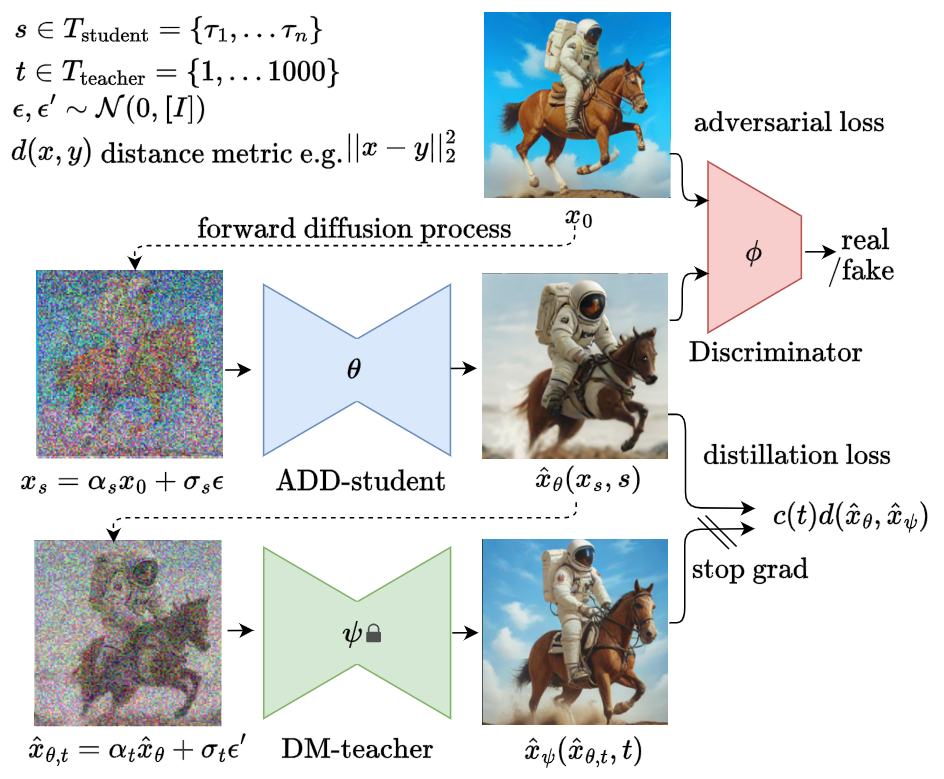
\includegraphics[width=\textwidth/2]{sdxlarchitecture.png}
    \caption{Architecture of the SDXL Turbo model.}
    \vspace{0.1cm}
    \label{fig:sdxlarchitecture}
\end{figure}

SDXL Turbo is capable of generating photorealistic images based on minimal input, such as a rough sketch or a short text prompt.
This efficiency is critical for the AI Totem platform, as it allows the system to quickly transform user drawings into detailed digital artwork without noticeable delays.
Despite the model's speed, it maintains high fidelity in the images it produces, capturing intricate details and textures that elevate the original sketch into something far more sophisticated.

Given that SDXL Turbo is memory-intensive, the Totem platform offloads the image generation process to a remote endpoint, allowing devices with limited hardware resources to still take advantage of the model's capabilities.
This approach ensures that users can access fast and detailed image generation without overloading the processing power of their devices.

\begin{figure}[h!]
    \centering
    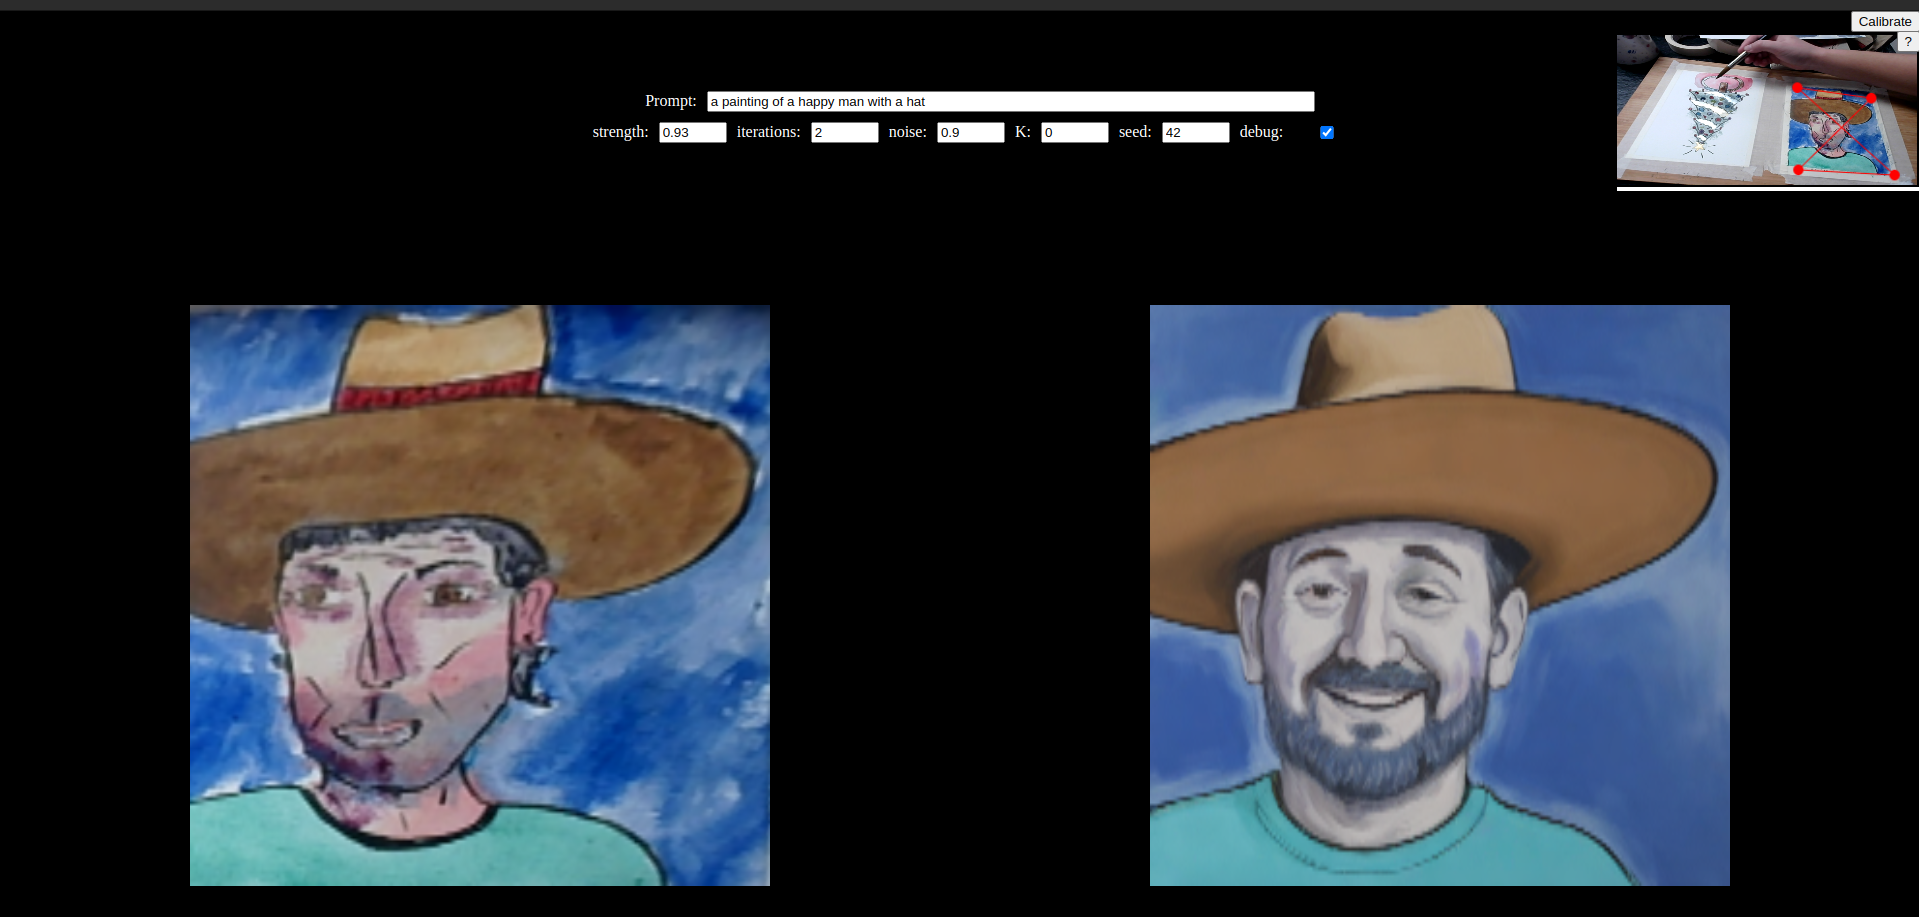
\includegraphics[width=\textwidth/3]{HatManhappy.png}
    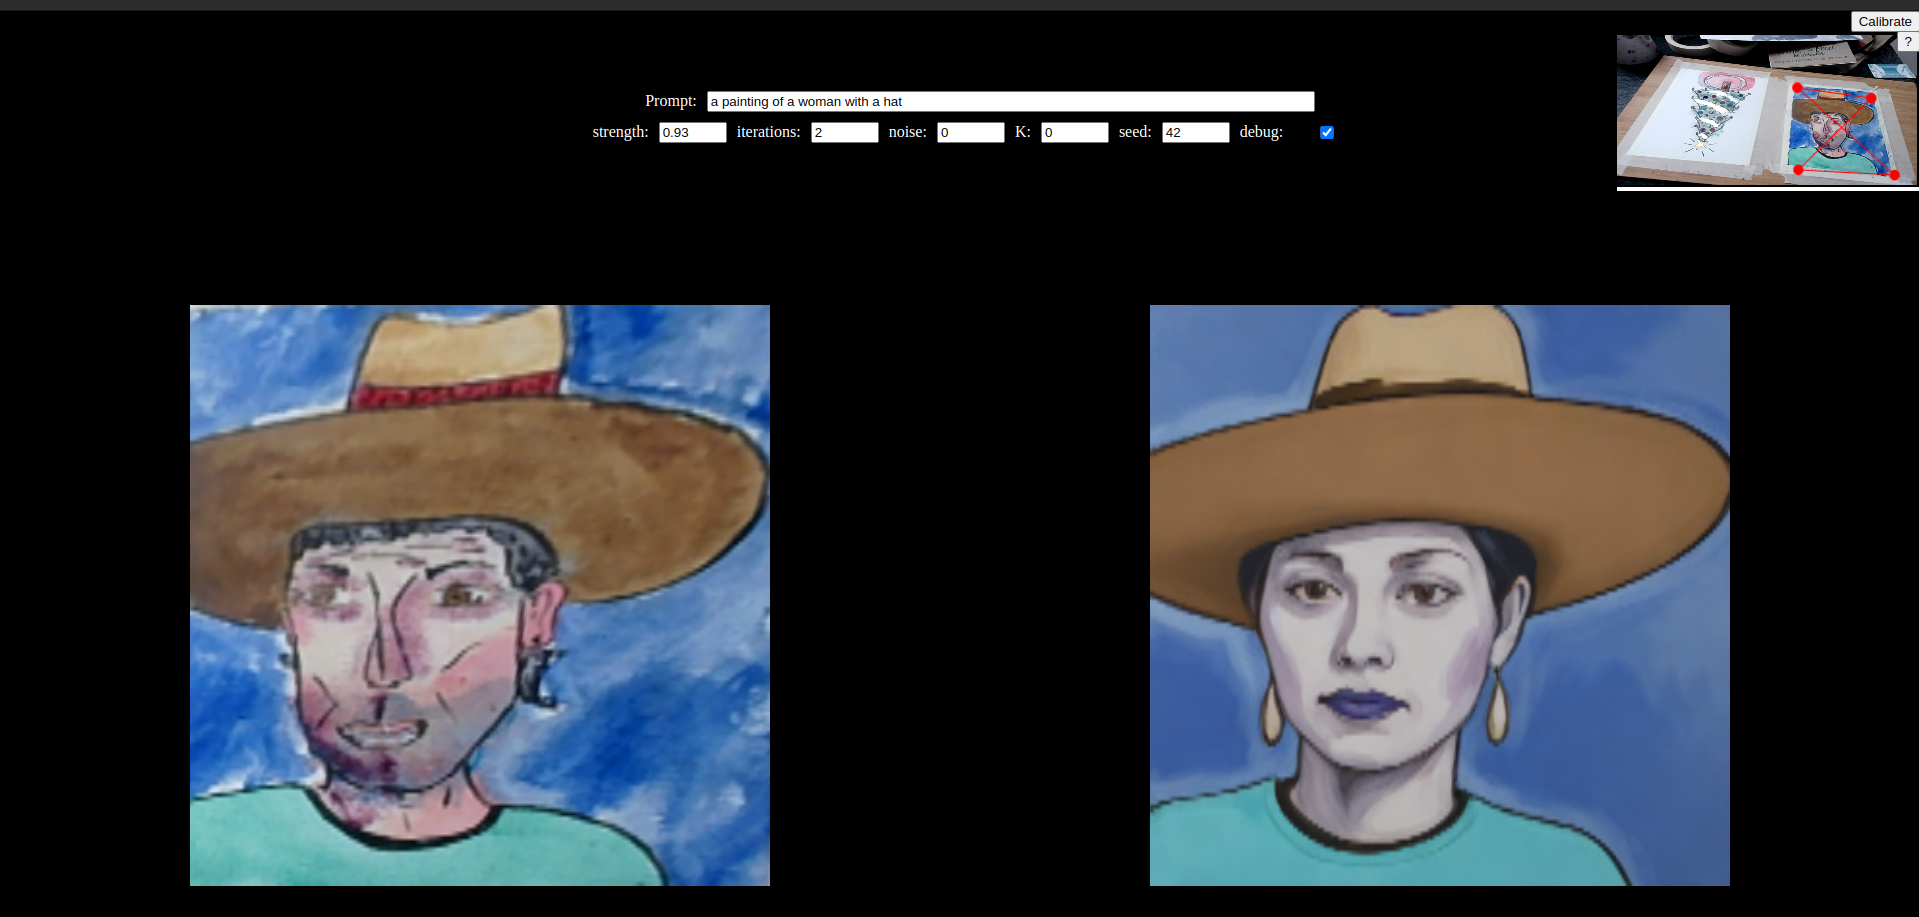
\includegraphics[width=\textwidth/3]{HatManwoman.png}
    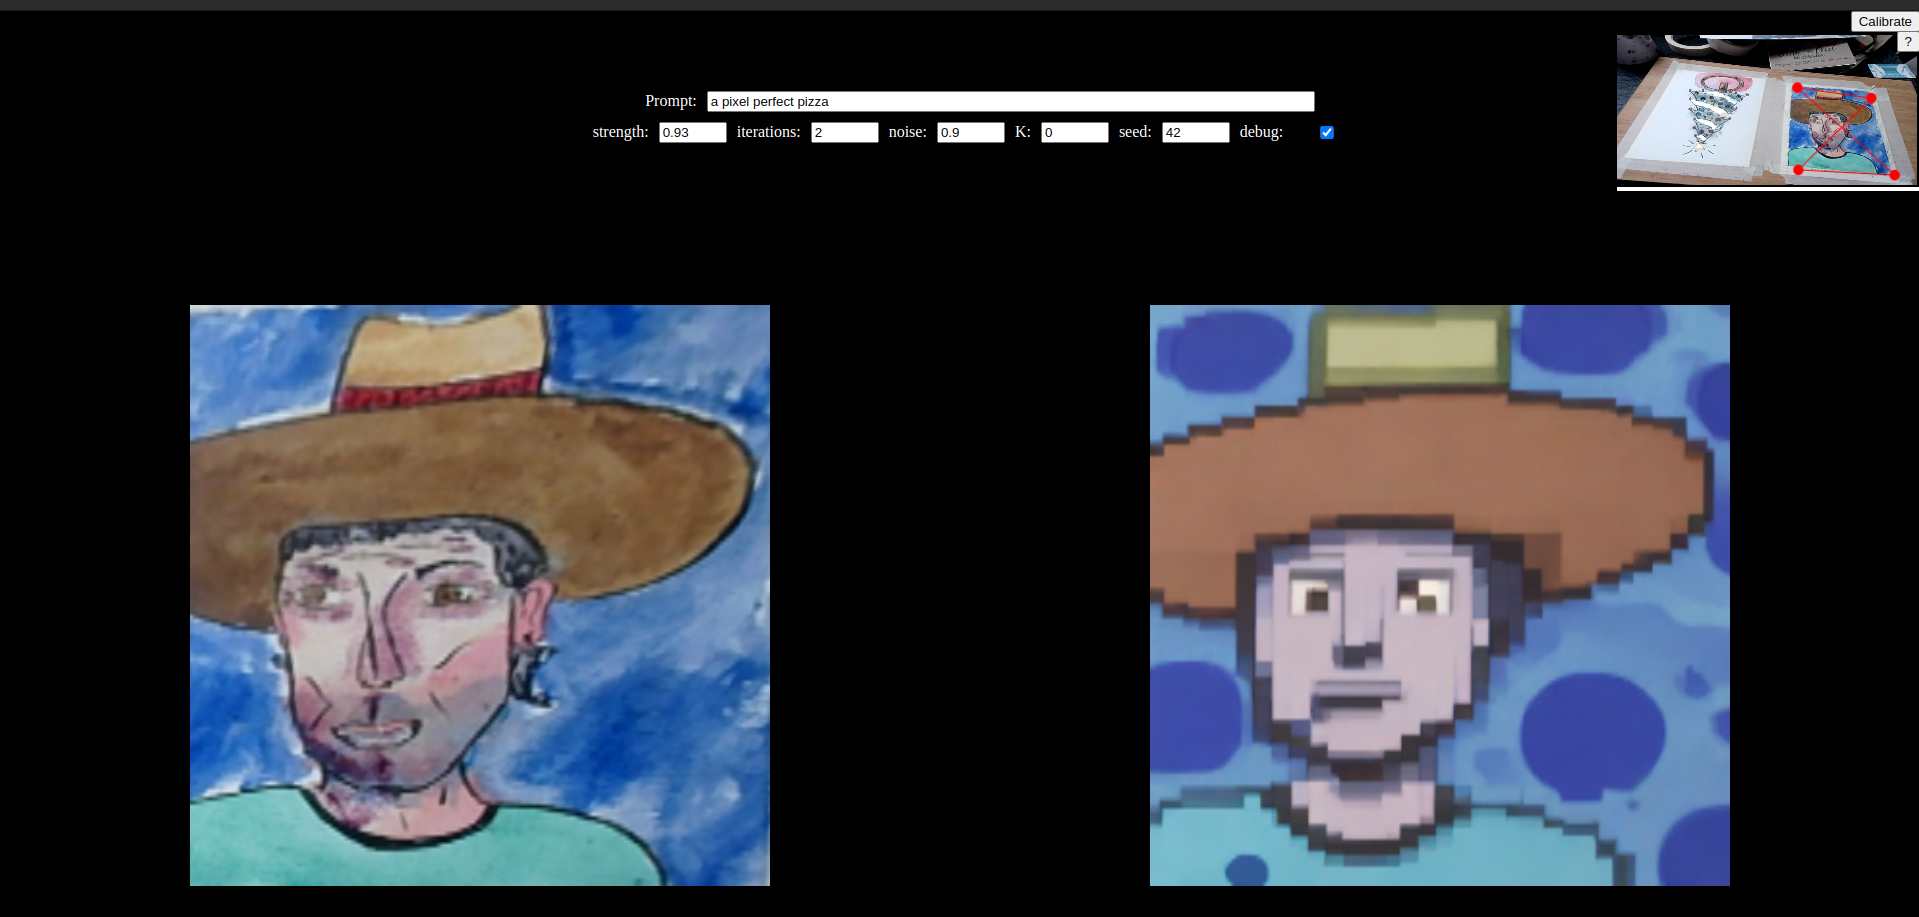
\includegraphics[width=\textwidth/3]{HatMancubes.png}
    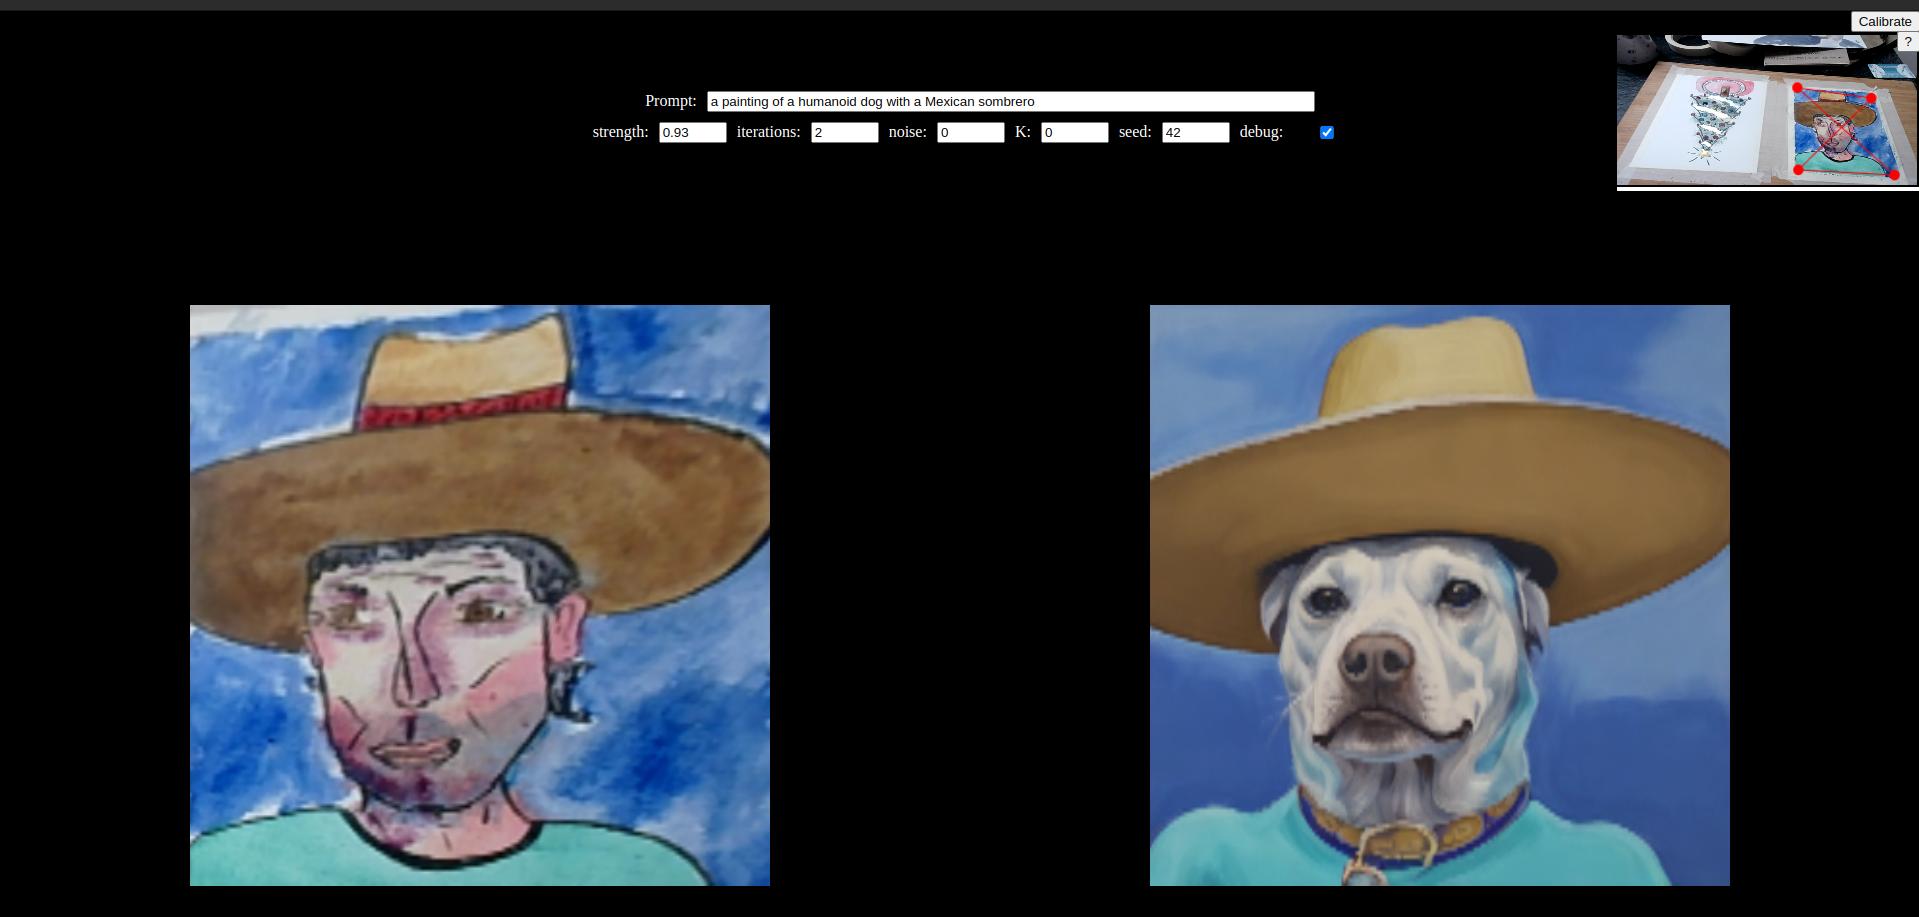
\includegraphics[width=\textwidth/3]{HatManDog.png}
    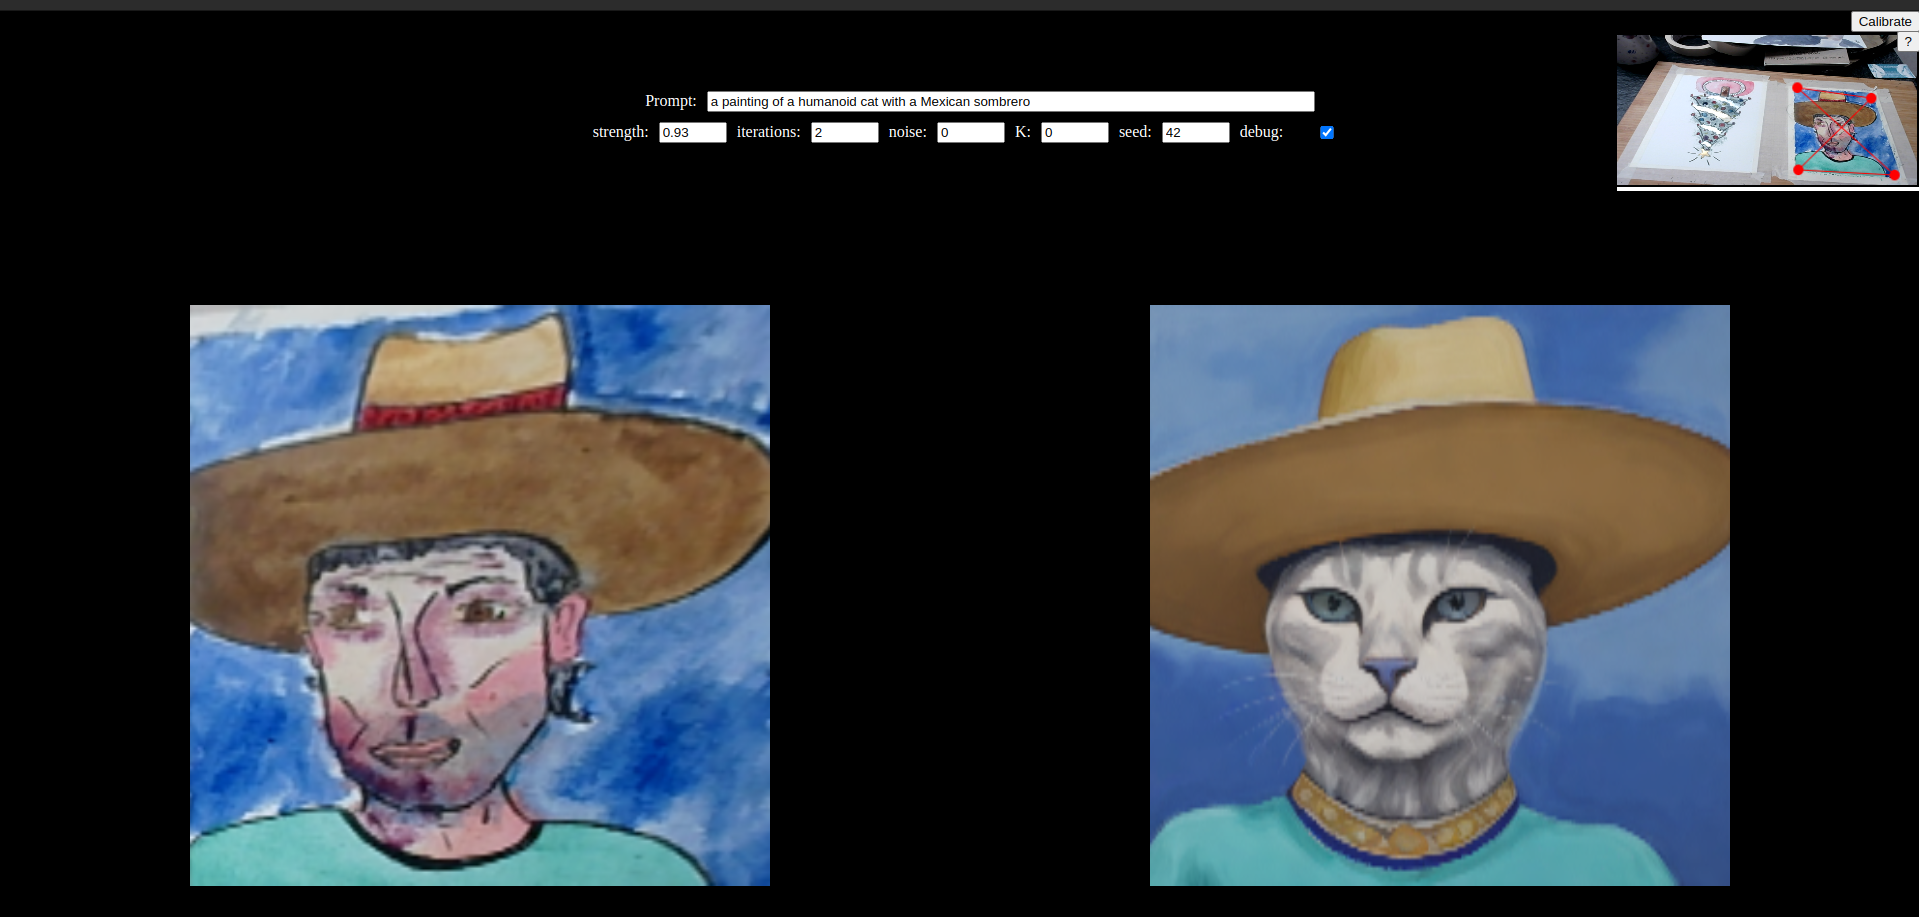
\includegraphics[width=\textwidth/3]{HatManCAT3.png}
    \caption{SDXL Turbo-generated images based on simple painting.}
    \vspace{0.1cm}
    \label{fig:sdxlpainting}
\end{figure}

\floatbarrier

\subsubsection{ How It All Comes Together}


The \textbf{AI Totem platform} ties these components together into a cohesive system that runs efficiently, even on resource-constrained devices.
To ensure smooth performance, the platform separates the processing of different tasks across multiple threads and systems:

\begin{figure}[h!]
    \centering
    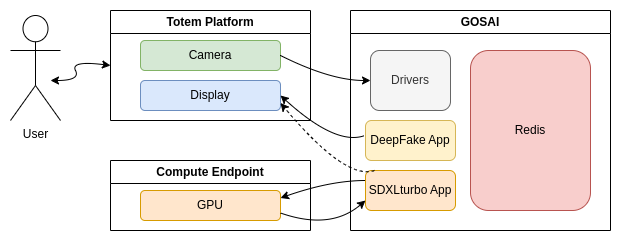
\includegraphics[width=\textwidth]{totemDiag.drawio.png}
    \caption{Architecture diagram of the AI Totem platform.}
    \vspace{0.1cm}
    \label{fig:diagtotem}
\end{figure}

1.  \textbf{Image Generation via Remote Endpoint}: Since \textbf{SDXL Turbo} is a memory-intensive model, it is hosted remotely and accessed via an API.
When a user submits a sketch, the platform sends the drawing to the remote endpoint, where SDXL Turbo quickly processes it and returns a high-quality image.
This offloading approach allows the platform to maintain fast image generation without burdening the local device, ensuring smooth user experiences.
    
\begin{figure}[h]
    \centering
    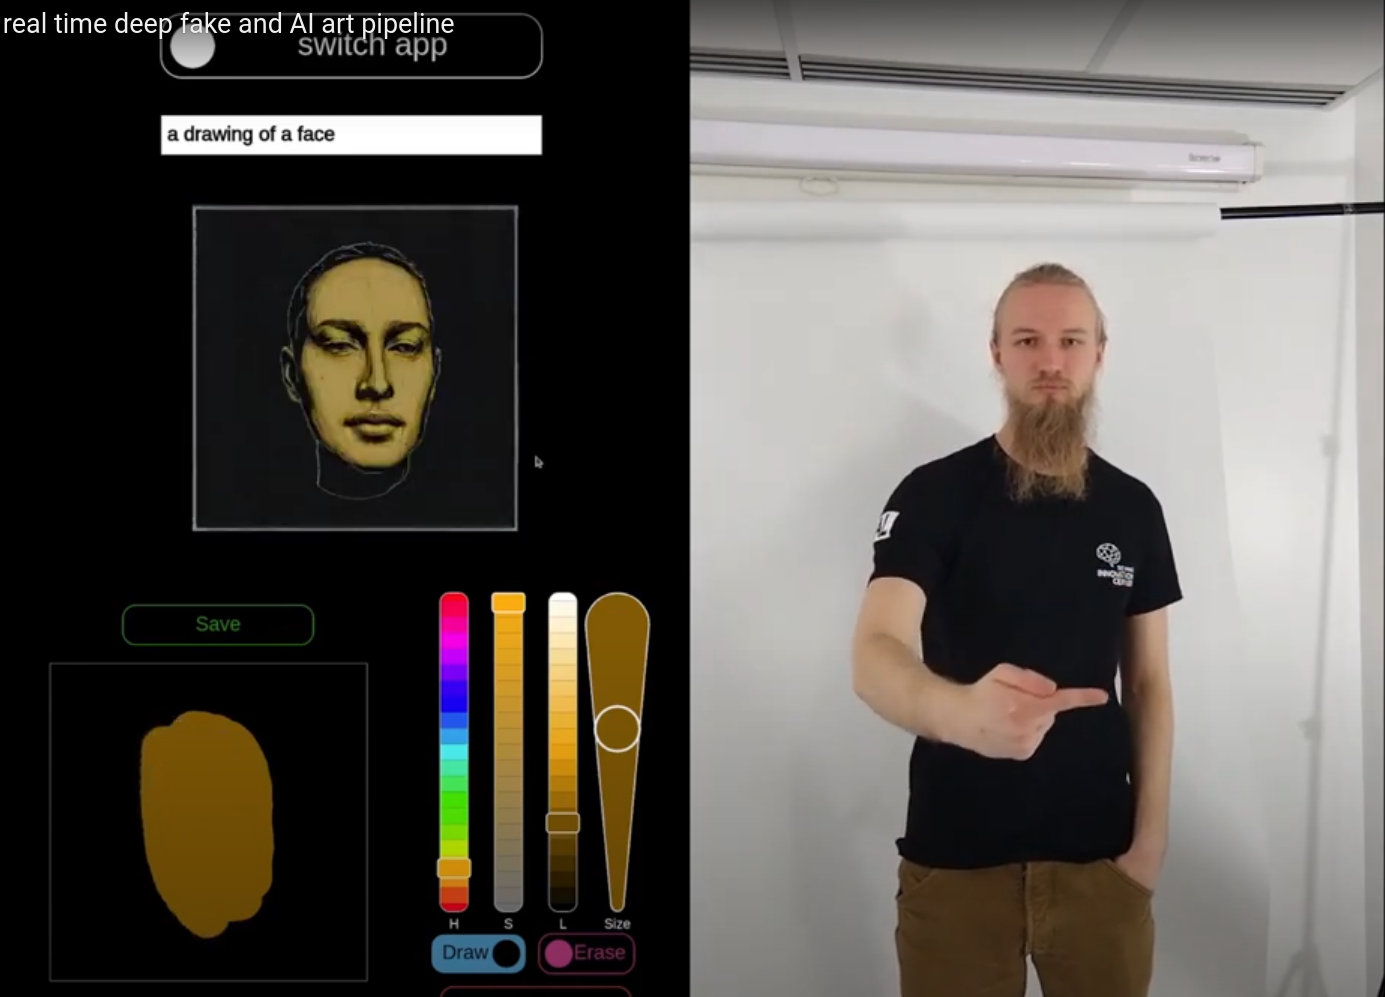
\includegraphics[width=\textwidth/2]{sdxlapp.png}
    \caption{Overview of the image generation app.}
    \vspace{0.1cm}
    \label{fig:imgenapp}
\end{figure}

2.  \textbf{Deepfake Animation in Real-Time}: The deepfake animation, powered by the \textbf{First Order Motion model}, runs directly on the device.
This is possible due to the model's relatively low computational requirements, which make it feasible to process the user's interactions and animate the AI-generated characters in real time.
GOSAI handles the interaction between the user's actions (such as head movements or gestures) and the animated characters, ensuring a seamless AR experience.

\begin{figure}[h]
    \centering
    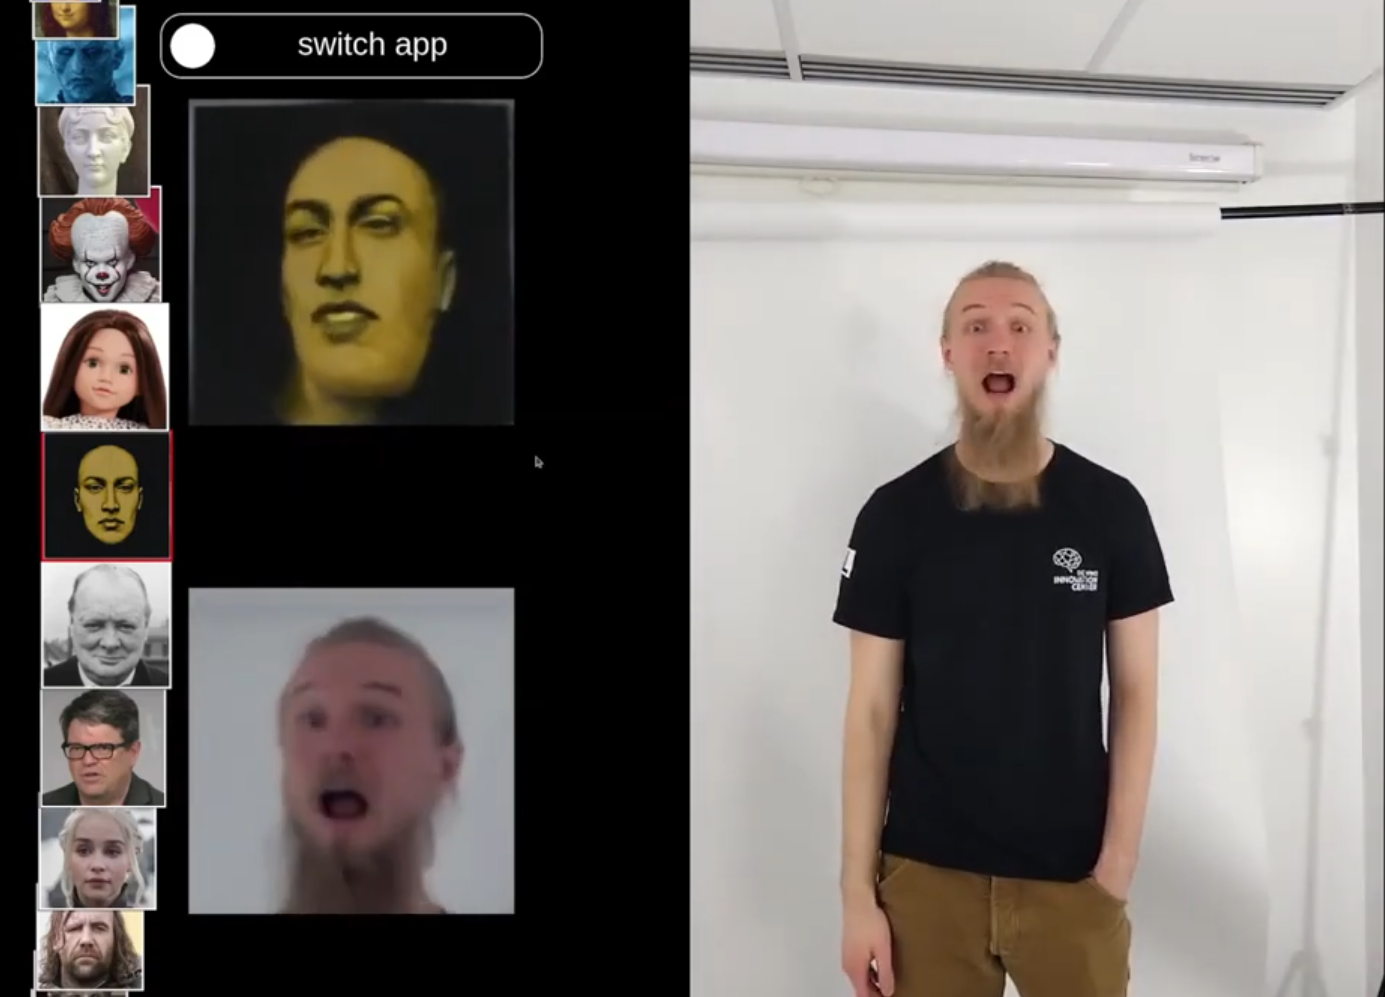
\includegraphics[width=\textwidth/2]{deepfakeapp.png}
    \caption{Overview of the deepfake app.}
    \vspace{0.1cm}
    \label{fig:deepfakeapp}
\end{figure}
    

By distributing the workload in this way, the AI Totem platform achieves a balance between \textbf{real-time interaction} and \textbf{high-quality image generation}, creating a fluid experience for users.
GOSAI manages the integration of these elements, allowing the system to run efficiently across different devices while maintaining a high level of interactivity and detail.



\subsection{Conclusion}

The \textbf{AI Totem platform} represents a convergence of Artificial Intelligence (AI) and Augmented Reality (AR), leveraging technologies like the \textbf{SDXL Turbo} diffusion model and the \textbf{First Order Motion} model.
This fusion transforms simple sketches into dynamic, animated creations, immersing users in an interactive AR environment powered by the \textbf{GOSAI framework}.

From a technical standpoint, the platform achieves a seamless integration of AI-driven generation and real-time AR interaction.
The implementation challenges—such as maintaining high image quality with fast response times—are addressed through strategic use of remote endpoints for image generation and local processing for animations.
This allows users to experience a fluid and responsive environment where creativity is enhanced by technology.

However, the platform’s success is not solely due to its technical efficiency.
Its true value lies in how it redefines the relationship between creators and their digital art.
By automating traditionally labor-intensive processes like detailed image generation and animation, AI Totem democratizes access to complex creative tools, lowering the barrier for users with limited technical expertise.

% The implementation of the \textbf{AI Totem platform} is a complex integration of AR and AI technologies, each contributing to the platform's ability to transform simple sketches into interactive, animated digital art.
% By leveraging the \textbf{GOSAI framework} for AR interaction, the \textbf{First Order Motion model} for deepfake animations, and \textbf{SDXL Turbo} for fast, high-quality image generation, the platform creates a dynamic environment where users can engage with their creations in real time.

% This combination of technologies not only enhances the creative process but also showcases how AI and AR can work together to push the boundaries of what is possible in digital art and HCI.
% The modular and scalable nature of the platform ensures that it can be adapted for various use cases, from interactive storytelling to educational tools, making AI Totem a powerful example of the future of creativity in the digital age.

\subsubsection{Discussion}

The AI Totem platform opens up several intriguing discussions in the field of Human-Computer Interaction (HCI).
First, it raises questions about the role of AI in creative processes.
While AI augments creativity by simplifying complex tasks, does it diminish the role of human intuition in artistic expression?
This balance between human creativity and machine assistance will continue to evolve as AI tools become more sophisticated and accessible.

Another critical discussion surrounds the use of AR as a medium for digital art.
AR offers a unique canvas where digital creations interact with the physical world.
The immersive and interactive capabilities of AR, when combined with AI, challenge traditional forms of storytelling and artistic engagement.
Yet, the success of such platforms relies on their usability—whether the system can offer powerful creative tools without overwhelming the user.
In this sense, AI Totem addresses this by abstracting much of the complexity through automation, but further research into improving user interfaces and experience could lead to even more intuitive systems.

Lastly, the platform also highlights the importance of performance optimization in real-time applications.
The comparison between frameworks like PyTorch, TorchScript, and ONNX demonstrated that even small improvements in latency or resource management can significantly impact user experience, particularly in mobile or resource-constrained environments.
This balancing act between quality, speed, and resource efficiency will be critical for future developments.

\subsubsection{Final Thoughts}

The \textbf{AI Totem platform} successfully bridges the gap between AI and AR, offering an accessible and immersive way to engage with digital art.
It highlights the potential of AI-driven tools to transform creative processes, making complex tasks more manageable while allowing users to focus on their artistic expression.
Moreover, by blending these technologies in real-time, the platform opens up new avenues for interactive storytelling and dynamic user experiences.

As the boundaries between AI, AR, and HCI continue to blur, projects like AI Totem pave the way for a future where digital creativity is no longer limited by technical constraints.
This project demonstrates that when integrated effectively, AI and AR can elevate both the creative process and the user experience, making it an essential tool in the evolving landscape of digital art and HCI.